% Options for packages loaded elsewhere
\PassOptionsToPackage{unicode}{hyperref}
\PassOptionsToPackage{hyphens}{url}
%
\documentclass[
  english,
  man]{apa7}
\usepackage{lmodern}
\usepackage{amssymb,amsmath}
\usepackage{ifxetex,ifluatex}
\ifnum 0\ifxetex 1\fi\ifluatex 1\fi=0 % if pdftex
  \usepackage[T1]{fontenc}
  \usepackage[utf8]{inputenc}
  \usepackage{textcomp} % provide euro and other symbols
\else % if luatex or xetex
  \usepackage{unicode-math}
  \defaultfontfeatures{Scale=MatchLowercase}
  \defaultfontfeatures[\rmfamily]{Ligatures=TeX,Scale=1}
\fi
% Use upquote if available, for straight quotes in verbatim environments
\IfFileExists{upquote.sty}{\usepackage{upquote}}{}
\IfFileExists{microtype.sty}{% use microtype if available
  \usepackage[]{microtype}
  \UseMicrotypeSet[protrusion]{basicmath} % disable protrusion for tt fonts
}{}
\makeatletter
\@ifundefined{KOMAClassName}{% if non-KOMA class
  \IfFileExists{parskip.sty}{%
    \usepackage{parskip}
  }{% else
    \setlength{\parindent}{0pt}
    \setlength{\parskip}{6pt plus 2pt minus 1pt}}
}{% if KOMA class
  \KOMAoptions{parskip=half}}
\makeatother
\usepackage{xcolor}
\IfFileExists{xurl.sty}{\usepackage{xurl}}{} % add URL line breaks if available
\IfFileExists{bookmark.sty}{\usepackage{bookmark}}{\usepackage{hyperref}}
\hypersetup{
  pdftitle={Web-CDI: A system for online administration of the MacArthur-Bates Communicative Development Inventories},
  pdfauthor={Benjamin deMayo1, Danielle Kellier2, Mika Braginsky3, Christina Bergmann4, Cielke Hendriks4, Caroline Rowland4, Michael C. Frank5, \& Virginia Marchman5},
  pdflang={en-EN},
  pdfkeywords={vocabulary development, parent report, socioeconomic status},
  hidelinks,
  pdfcreator={LaTeX via pandoc}}
\urlstyle{same} % disable monospaced font for URLs
\usepackage{graphicx,grffile}
\makeatletter
\def\maxwidth{\ifdim\Gin@nat@width>\linewidth\linewidth\else\Gin@nat@width\fi}
\def\maxheight{\ifdim\Gin@nat@height>\textheight\textheight\else\Gin@nat@height\fi}
\makeatother
% Scale images if necessary, so that they will not overflow the page
% margins by default, and it is still possible to overwrite the defaults
% using explicit options in \includegraphics[width, height, ...]{}
\setkeys{Gin}{width=\maxwidth,height=\maxheight,keepaspectratio}
% Set default figure placement to htbp
\makeatletter
\def\fps@figure{htbp}
\makeatother
\setlength{\emergencystretch}{3em} % prevent overfull lines
\providecommand{\tightlist}{%
  \setlength{\itemsep}{0pt}\setlength{\parskip}{0pt}}
\setcounter{secnumdepth}{-\maxdimen} % remove section numbering
% Make \paragraph and \subparagraph free-standing
\ifx\paragraph\undefined\else
  \let\oldparagraph\paragraph
  \renewcommand{\paragraph}[1]{\oldparagraph{#1}\mbox{}}
\fi
\ifx\subparagraph\undefined\else
  \let\oldsubparagraph\subparagraph
  \renewcommand{\subparagraph}[1]{\oldsubparagraph{#1}\mbox{}}
\fi
% Manuscript styling
\usepackage{upgreek}
\captionsetup{font=singlespacing,justification=justified}

% Table formatting
\usepackage{longtable}
\usepackage{lscape}
% \usepackage[counterclockwise]{rotating}   % Landscape page setup for large tables
\usepackage{multirow}		% Table styling
\usepackage{tabularx}		% Control Column width
\usepackage[flushleft]{threeparttable}	% Allows for three part tables with a specified notes section
\usepackage{threeparttablex}            % Lets threeparttable work with longtable

% Create new environments so endfloat can handle them
% \newenvironment{ltable}
%   {\begin{landscape}\begin{center}\begin{threeparttable}}
%   {\end{threeparttable}\end{center}\end{landscape}}
\newenvironment{lltable}{\begin{landscape}\begin{center}\begin{ThreePartTable}}{\end{ThreePartTable}\end{center}\end{landscape}}

% Enables adjusting longtable caption width to table width
% Solution found at http://golatex.de/longtable-mit-caption-so-breit-wie-die-tabelle-t15767.html
\makeatletter
\newcommand\LastLTentrywidth{1em}
\newlength\longtablewidth
\setlength{\longtablewidth}{1in}
\newcommand{\getlongtablewidth}{\begingroup \ifcsname LT@\roman{LT@tables}\endcsname \global\longtablewidth=0pt \renewcommand{\LT@entry}[2]{\global\advance\longtablewidth by ##2\relax\gdef\LastLTentrywidth{##2}}\@nameuse{LT@\roman{LT@tables}} \fi \endgroup}

% \setlength{\parindent}{0.5in}
% \setlength{\parskip}{0pt plus 0pt minus 0pt}

% \usepackage{etoolbox}
\makeatletter
\patchcmd{\HyOrg@maketitle}
  {\section{\normalfont\normalsize\abstractname}}
  {\section*{\normalfont\normalsize\abstractname}}
  {}{\typeout{Failed to patch abstract.}}
\patchcmd{\HyOrg@maketitle}
  {\section{\protect\normalfont{\@title}}}
  {\section*{\protect\normalfont{\@title}}}
  {}{\typeout{Failed to patch title.}}
\makeatother
\shorttitle{Web-CDI}
\keywords{vocabulary development, parent report, socioeconomic status\newline\indent Word count: X}
\DeclareDelayedFloatFlavor{ThreePartTable}{table}
\DeclareDelayedFloatFlavor{lltable}{table}
\DeclareDelayedFloatFlavor*{longtable}{table}
\makeatletter
\renewcommand{\efloat@iwrite}[1]{\immediate\expandafter\protected@write\csname efloat@post#1\endcsname{}}
\makeatother
\usepackage{lineno}

\linenumbers
\usepackage{csquotes}
\ifxetex
  % Load polyglossia as late as possible: uses bidi with RTL langages (e.g. Hebrew, Arabic)
  \usepackage{polyglossia}
  \setmainlanguage[]{english}
\else
  \usepackage[shorthands=off,main=english]{babel}
\fi

\title{Web-CDI: A system for online administration of the MacArthur-Bates Communicative Development Inventories}
\author{Benjamin deMayo\textsuperscript{1}, Danielle Kellier\textsuperscript{2}, Mika Braginsky\textsuperscript{3}, Christina Bergmann\textsuperscript{4}, Cielke Hendriks\textsuperscript{4}, Caroline Rowland\textsuperscript{4}, Michael C. Frank\textsuperscript{5}, \& Virginia Marchman\textsuperscript{5}}
\date{}


\affiliation{\vspace{0.5cm}\textsuperscript{1} Princeton University\\\textsuperscript{2} University of Pennsylvania\\\textsuperscript{3} Massachussetts Institute of Technology\\\textsuperscript{4} Max Planck Institute for Psycholinguistics\\\textsuperscript{5} Stanford University}

\abstract{
Understanding the mechanisms which drive variation in children's language acquisition requires large, population-representative datasets of children's word learning across development. Parent report measures such as the MacArthur-Bates Communicative Development Inventories (CDI) are commonly used to accrue such data, but the traditional paper-based forms make the curation of large datasets logistically challenging, and tend to rely on convenience samples located close in proximity to major research institutions. Here, we introduce Web-CDI, a web-based tool which allows researchers to collect CDI data online. Web-CDI contains functionality to collect and manage longitudinal data, share links, and download standardized vocabulary scores. To date, over 3,500 valid Web-CDI administrations have been completed. General trends found in past norming studies of the CDI are present in data collected from Web-CDI: scores of children's productive vocabulary grow with age, female children show a slightly faster rate of vocabulary growth in early childhood, and participants with higher levels of education attainment report slightly higher vocabulary production scores. We also report results from an effort to oversample non-white, lower-SES participants (N = 241), which showed similar demographic trends to the full sample but which had a high exclusion rate. Implications and challenges for the collection of large, population-representative datasets using Web-CDI in future research are discussed.
}



\begin{document}
\maketitle

Children vary tremendously in their vocabulary development (Frank, Braginsky, Yurovsky, \& Marchman, 2021). Characterizing this variability is central to understanding the mechanisms that drive early language acquisition, yet capturing this variation in broad, diverse samples of children has been a significant challenge for cognitive scientists for decades. The MacArthur-Bates Communicative Development Inventory (MB-CDI, or CDI for short) is a commonly-used parent report instrument for assessing vocabulary development in early childhood (Fenson et al., 2007) that was introduced in part to create a cost-effective method for measuring variability across individuals.

In this paper, we introduce a web-based tool, Web-CDI, developed to address the need for collecting CDI data in an online format. Web-CDI allows researchers to increase the convenience of CDI administration, further decrease costs associated with data collection and entry, and access participant samples that have traditionally been difficult to reach in language development research. Our purpose in this paper is twofold: first, we describe Web-CDI as a platform which streamlines the process of collecting MB-CDI data and collates the data in a way that facilitates the creation of large-scale, multisite collaborative datasets. Second, we profile usage of Web-CDI thus far, with a particular focus on broadening the reach of traditional paper-based methods of collecting vocabulary development data.

We begin by discussing parent report as a powerful method by which to address the challenge of measuring early language outcomes, as well as previous online parent report instruments. We then describe Web-CDI and its use from the perspective of participants and researchers. Finally, we report on our use of Web-CDI thus far and discuss the potential of Web-CDI to acquire vocabulary data from diverse, population-representative samples. We end with some challenges for future research.

\hypertarget{the-importance-of-parent-report-data}{%
\subsection{The Importance of Parent Report Data}\label{the-importance-of-parent-report-data}}

Gaining empirical traction on variation in children's early language requires reliable and valid methods for measuring language abilities, especially in early childhood (8 to 30 months). Parent report is a mainstay in this domain. Parent reports are based on their daily experiences with the child, which are much more extensive than a researcher or clinician can generally obtain. Moreover, they are less likely to be influenced by factors that may mask a child's true ability in the laboratory or clinic (e.g., shyness; Frank et al. (2021)), and parents are remarkably accurate at reporting their children's language, especially in the first two years of life (CITE). One widely used set of parent-report instruments is the MacArthur-Bates Communicative Development Inventories, originally designed for children learning American English (Fenson et al., 2007). The American English CDIs come in two versions, Words \& Gestures for children 8 to 18 months, focusing on word comprehension and production, as well as gesture use, and Words \& Sentences, for children 16 to 30 months, focusing on word production and sentence structure. Together, these instruments allow for a comprehensive picture of milestones that characterize language development in the first 2½ years of life.

A substantial body of evidence suggests that these instruments are both reliable and valid (e.g., Fenson et al., 1994, 2007) leading to their widespread use in thousands of research studies over the last few decades. Indeed, the popularity of the American English and Spanish CDI instruments has meant that many teams around the world have adapted the CDI format to the particular language and community (Dale, 2015). Importantly, these adaptations are not simply translations of the original form but rather incorporate the specific features of different languages and cultures, since linguistic variability exists even among cultures that share a native language (e.g., Cheerios are more common in American than British homes, so age of acquisition of this word may differ substantially). To date there are now more than 100 adaptations for languages around the globe.

Initial large-scale work to establish the normative datasets for the American English CDI not only provided key benchmarks for determining children's progress, but also documented the extensive individual differences that characterize early language learning during this critical period of development (Bates et al., 1994; Fenson et al., 1994). Understanding the origins and consequences of this variability remains an important empirical and theoretical endeavor that has informed critical insights in the field (e.g., Bates \& Goodman, 2001; Bornstein \& Putnick, 2012; see also, Frank et al., 2021). The popularity of the instruments has remained strong over the years, leading to the development of extensions of the methodology to alternative formats, e.g., short forms (Fenson et al., 2000).

While the reliability and validity of these instruments is well-established (Fenson et al., 2007) for the American English versions of the forms, existing norming samples are skewed toward families with more years of formal education and away from non-White groups. Representation in the norming samples is generally restricted to families living on the US east and west coasts (CITE FOR THIS). Further, although paper survey administration is a time-tested method, increasingly researchers and participants would prefer to use an electronic method to administer and fill CDI forms, obviating the need to track (and sometimes mail) paper forms, and the need to key in hundreds of item-wise responses for each child.

Here, we report on our recent efforts to create and distribute a web-based version of the MacArthur-Bates CDIs in order to address some of the limitations of the standard paper versions. Online administration of the CDI is not a novel innovation -- a variety of research groups have created purpose-build platforms for administering the CDI in particular languages. For example, Kristoffersen et al. (2013) collected a large normative sample of Norwegian CDIs using a custom online platform. Similarly, the Slovak adaptation of the CDI uses an online administration format (CHECK CITE HERE). And many groups have used general purpose survey software such as Qualtrics and Survey Monkey to administer CDIs and variants online (e.g., Caselli, Lieberman, and Pyers (2020)). The innovation of Web-CDI is to provide a comprehensive researcher management interface for the administration of a wide range of CDI forms, allowing researchers to manage longitudinal administrations, download standardized scores, and share links easily, all while satisfying strong guarantees regarding privacy and anonymity. Moreover, a key benefit of a unified data collection and storage system such as Web-CDI is that data from disparate sources are combined into a single repository, far reducing the overhead efforts associated with bringing together data collected using paper forms by researchers across the world.

\hypertarget{introducing-web-cdi}{%
\subsection{Introducing Web-CDI}\label{introducing-web-cdi}}

Web-CDI is our web-based platform for CDI administration and management. Parents are recruited by either receiving an individual URL directly from a researcher or by interacting with a targeted social media advertisement using general-purpose URLs. Web-CDI serves as a low-risk method that allows researchers to communicate with families electronically, facilitating access to families in areas distant from an academic institution and eliminating costly mailings or laboratory visits. It also permits other institutions to use Web-CDI as a resource, while still allowing members of the CDI Advisory Board to access and analyze the resulting data with the researchers' permissions. Since 2018, more than 3000 CDIs have been collected via 15 research groups throughout the US, demonstrating the potential for large-scale data collection and aggregation.

Below, we outline how Web-CDI is used. We begin by detailing the consent obtention process and participant experience. Second, we describe the interface that researchers use to collect data using Web-CDI, specifying a number of common use cases for the platform. Lastly, we briefly discuss the administrator role.

\hypertarget{participant-interface}{%
\subsubsection{Participant interface}\label{participant-interface}}

Participants can complete the Web-CDI on a variety of devices, including personal computers and tablets; Web-CDI can be administered on a smartphone, although the experience is not as ideal for the user due to the length of the survey. When a participant clicks a link to the form, they are directed to a website displaying their own personal administration of the Web-CDI, regardless of whether the link was participant-specific or general-purpose. In some cases, they may be asked to read and accept a waiver of consent documentation, depending on whether the researcher has chosen to use that feature (see also Researcher Interface below).

\emph{Demographics.} The parent is then asked to provide demographic information about their family and any health conditions that might impact their child's vocabulary development. The specific demographic questions asked of participants can be adjusted to vary between different versions of the form, allowing researchers to tailor the demographic questions to local norms\footnote{For example, the Dutch CDI omits questions about participant ethnicity, since census data in the Netherlands does not include ethnicity.}. Researchers can customize the presentation of these demographic questions in three ways. First, they can elect to show all of the demographics items on the landing page or they elect to present the majority of these questions at the end of the instrument. This choice is provided because some pilot work in the United Kingdom indicated that answering questions regarding personal health information at the beginning may deter participants from completing the instrument. Second, certain demographic questions can be asked at both the beginning and the end of the form to serve as validity checks, providing a check that can be used to screen for hasty or illegitimate completions. Third, researchers can tailor the questions to the societal and cultural context of their participants (e.g.~country-specific education level descriptors and income categories).

\begin{figure}
\centering
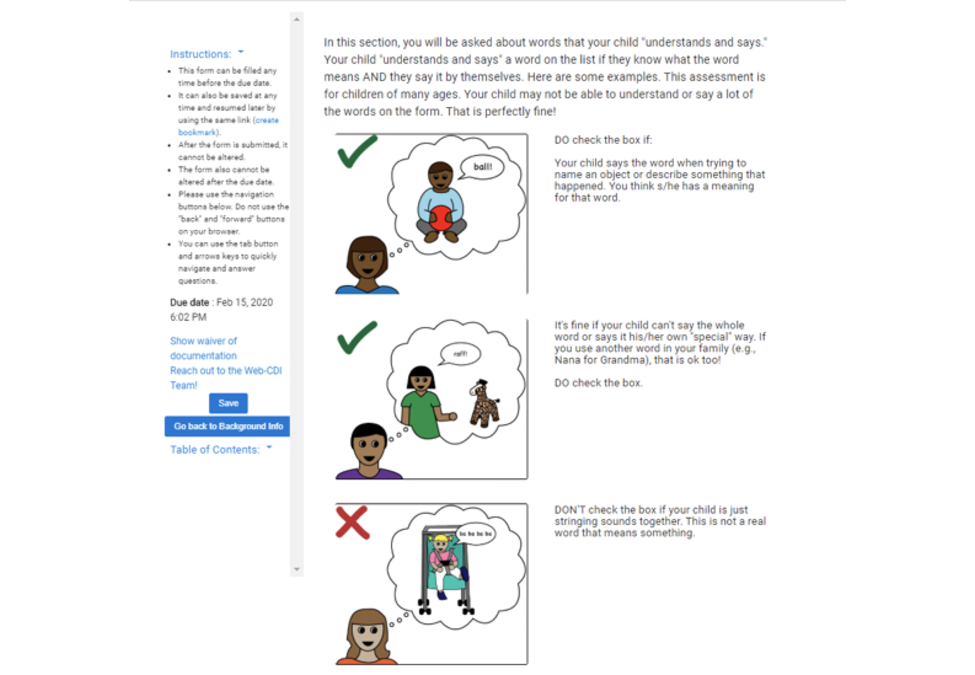
\includegraphics{webcdi_paper_files/figure-latex/pictorial-1.pdf}
\caption{\label{fig:pictorial}Pictorial instructions in the Web-CDI Words and Sentences instrument.}
\end{figure}

\emph{Instructions.} After completing the first demographics page, participants are directed to the instructions that are appropriate for either the Words \& Gestures or Words \& Sentences version (see Figure \ref{fig:pictorial}). At the top of the page are general instructions that inform participants that they should expect the study to take at least 30 minutes and that they should try to complete it in a quiet setting( e.g., while their child is sleeping). In addition, there are more detailed instructions for completing the vocabulary checklist. Unlike the traditional paper versions, instructions on how to properly choose responses are provided both in written and pictorial form. The pictorial instructions (Figure 1) aim to further increase caregivers' understanding of how to complete the checklist. For example, these instructions clarify that the child's understanding of a word requires them to have some understanding of the object that the word refers to or some aspect of the word's meaning. In addition, caregivers are reassured that \enquote{child like} forms (e.g., \enquote{raff} for \enquote{giraffe}) or family- or dialect-specific forms (e.g., \enquote{nana} for \enquote{grandma} are acceptable). Lastly, caregivers are reminded that the child should be able to produce the words \enquote{on their own} and that imitations are not acceptable. These general \enquote{rules of thumb} for completing the form should be familiar to researchers who are distributing the forms to parents so they can field any questions that may arise. While this is not possible for certain use-cases (e.g., collecting data via Facebook), these instructions should ideally also be reviewed either in writing (e.g., via email) or verbally (e.g., over the phone), so that these pictured instructions serve merely as a reminder to caregivers when completing the form.

\emph{Completing the instrument.} The majority of the participant's time in the study is spent completing the main sections of the instruments. As shown in Figure 2, on the American English Words and Gestures form, the vocabulary checklist portion of the form (396 items) asks parents to indicate whether their child can \enquote{understand} or \enquote{understand and say} each word. Gesture communication and other early milestones are also assessed. In the American English Words and Sentences form, the vocabulary checklist (680 items) only asks parents to indicate which words their child \enquote{says}. Additional items assess children's production of their three longest sentences, as well as morphological and syntactic development more broadly.

At the completion of the form, a graph is displayed illustrating the proportion of words from each semantic category that the child currently produces or understands. In addition, data from the norming studies are used to estimate the \enquote{hardest} (i.e., most advanced) word that the child currently understands or produces. This feedback to parents is intended to provide parents with a fun \enquote{thank you} and is intentionally not designed to provide specific feedback about their child's progress. The closing page also reminds parents that their participation does not constitute a clinical evaluation and that they should contact their pediatrician or primary care physician if they have any concerns about their child's development.

\hypertarget{researcher-interface}{%
\subsubsection{Researcher Interface}\label{researcher-interface}}

\begin{longtable}[t]{>{\raggedright\arraybackslash}p{2.2in}>{\raggedright\arraybackslash}p{1in}>{\raggedright\arraybackslash}p{2.2in}}
\caption{\label{tab:unnamed-chunk-1}Settings customizable by researchers when creating new studies to be run on the Web-CDI platform.}\\
\toprule
\textbf{Study setting} & \textbf{Default value } & \textbf{Notes}\\
\midrule
\endfirsthead
\caption[]{\label{tab:unnamed-chunk-1}Settings customizable by researchers when creating new studies to be run on the Web-CDI platform. \textit{(continued)}}\\
\toprule
\textbf{Study setting} & \textbf{Default value } & \textbf{Notes}\\
\midrule
\endhead

\endfoot
\bottomrule
\endlastfoot
Study name & none & NA\\
Instrument & none & NA\\
Number of days before study expiration & 14 & Must be between 1 and 28 days.\\
Measurement units for birth weight & Pounds and ounces & Weight can also be measured in kilograms (kg).\\
Minimum time (minutes) a parent must take to complete the study & 6 & NA\\
Waiver of documentation & blank & Can be filled in by researchers to include a Waiver of Documentation for the participant to approve before proceeding to the experiment.\\
Pre-fill data for longitudinal participants? & “No, do not populate any part of the form” & Researchers can choose to pre-fill the background information and the vocabulary checklist.\\
Would you like to pay subjects in the form of Amazon gift cards? & No & If checked, researchers can enter gift codes to distribute to participants once they have completed the survey.\\
Do you plan on collecting only anonymous data in this study? (e.g., posting ads on social media, mass emails, etc) & No & If checked, researchers can set a limit for the maximum number of participants, as well as select an option that asks participants to verify that the information entered is accurate.\\
Would you like to show participants graphs of their data after completion? & Yes & NA\\
Would you like participants to be able to share their Web-CDI results via Facebook? & No & NA\\*
\end{longtable}

One of the main goals of Web-CDI is to facilitate wide distribution of the platform to the child language research community. To that end, researchers are required to contact a member of the CDI Advisory Board to register an account on Web-CDI, from which they can create studies to distribute to participants. Note that we ask that researchers allow fully anonymised data to be shared with us, so that it can be added to Wordbank (\url{http://wordbank.stanford.edu/}). However, there is an opt-out option if researchers do not wish to share their data.

A study in the context of the Web-CDI system is a set of individual administrations created by a researcher that share certain specifications. Table 1 gives an overview of the customizable features that are available at the study level in Web-CDI. These features are set when creating a study for the first time in Web-CDI using the \enquote{Create Study} tool, and most of the features can be updated continuously during data collection using the \enquote{Update Study} tool. While some of these features are only particularly relevant to specific use cases (e.g., longitudinal research and social media data collection, outline below), others are relevant to all researchers using Web-CDI.

There are currently several forms available for distribution on Web-CDI, including multiple versions of the English WG and WS forms and forms in other languages (see Cross-linguistic research below). When creating a study, researchers choose one of the forms that they would like to distribute to participants; only one can be used in a given study. Researchers who wish to send multiple forms to participants simultaneously (e.g., those conducting multilingual research) should create multiple studies, each with a single instrument associated with it.

Researchers can download participant data in two formats. Both formatting options output a comma-separated values file with one row per participant; the full data option includes participant-by-item responses, and allows researchers to explore item-level trends, while the summary data option omits item-level data and only provides summary scores (e.g., total number of words understood/produced, percentile scores by age and gender).

Below, we outline several possible use cases of Web-CDI, as well the features which may facilitate them from a researcher's perspective.

\emph{Individual recruitment.} One possible workflow using Web-CDI is to send unique study URLs to individual participants. Researchers do so by entering numerical participant IDs or by auto-generating a specified quantity of participant IDs, each with its own unique study URL, using the \enquote{Add Participants} tool in the researcher dashboard. New participants can be added on a continual basis so that researchers can adjust the sample size of their study during data collection. Unique links generated for individual participants expire, by default, 14 days after creation, though the amount of days before link expiration is adjustable, which may be an important consideration for some researchers depending on their participant populations and specific project timelines. This workflow is most suitable for studies which pair the CDI with other measures, or when researchers contact specific participants from an existing database.

\emph{Longitudinal studies.} Web-CDI also facilitates longitudinal study designs in which each participant completes multiple administrations. Researchers wishing to design longitudinal studies can do so by entering a list of meaningful participant IDs using the \enquote{Add Participants} tool in the researcher dashboard. If a certain participant ID is added multiple times, Web-CDI will create multiple unique study URLs in the study dashboard that have the same specified ID. In addition, when creating studies, researchers can select whether they would like the demographics information, vocabulary checklist, or no sections at all to be prefilled when a participant fills out a repeat administration of the instrument. Unless researchers are interested in cumulative vocabulary counts, it is strongly recommended that they do not use the option to pre-fill the vocabulary checklist portion of the instrument in longitudinal administrations as parents should complete the instrument at each time point independently.

\emph{Social media and survey vendors.} Web-CDI contains several features designed to facilitate data collection from social media recruitment or through third-party crowd-sourcing applications and vendors (e.g., Amazon Mechanical Turk, Prolific). First, rather than creating unique survey links for each participant, researchers can also use a single, anonymous link. When a participant clicks the anonymous link, a new administration with a unique subject ID is created in the study dashboard. Additionally, Web-CDI studies have several customizable features that are geared towards anonymous online data collection. For example, researchers can adjust the minimum amount of time a participant must take to fill out the survey before they are able to submit; with a longer minimum time to completion, researchers can encourage a more thorough completion of the survey. Researchers can also ask participants to verify that their information is accurate by checking a box at the end of the survey, and can opt to include certain demographic questions at both the beginning and end of the survey, using response consistency on these redundant items as a check of data quality.

\emph{Paid participation.} If researchers choose to compensate participants directly through the Web-CDI interface, Web-CDI has built-in functionality to distribute redeemable gift codes when a participant reaches the end of the survey. Web-CDI contains several features to facilitate integration with third-party crowdsourcing applications and survey vendors should they choose to handle participant compensation through another platform. For example, when creating studies, researchers can enter a URL to redirect participants to when they reach the end of the survey. Researchers using the behavioral research platform Prolific can configure their study to collect participants' unique Prolific IDs and pre-fill them in the survey.

\emph{Cross-linguistic research.} Web-CDI forms are currently available in English (U.S. American and Canadian), Spanish, French (Quebecois), Hebrew, Dutch and Korean. We are looking to add more language forms to the tool as the paper version of the forms has been adapted into more than 100 different languages and further ongoing adaptations have been approved by the MB-CDI board (\url{http://mb-cdi.stanford.edu/adaptations}).

\hypertarget{administrator-interface}{%
\subsubsection{Administrator Interface}\label{administrator-interface}}

System administrators who oversee the development and usage of Web-CDI can log into a specific interface provided by Django, the open-source web framework used to develop Web-CDI. This Django interface gives access to the entire dataset collected by all participating researchers, as well as all of the instrument forms that can be distributed to participants. Administrators approve new researchers' requests to create accounts on Web-CDI, and give individual researchers access to specific instrument forms. As an example, if a researcher wants to distribute the Spanish Words and Gestures form to participants, an administrator would need to give a researcher access to this instrument. Administrator privileges are limited to a handful of individuals, as most of the functionality accessible to administrators is not relevant to researchers using the survey for their own purposes.

\hypertarget{system-design}{%
\subsubsection{System Design}\label{system-design}}

Web-CDI is constructed using open-source software. All of the vocabulary data collected in Web-CDI are stored in a standard MySQL relational database, managed using Django and Python and hosted by Amazon Web Services. Individual researchers can download data from their studies through the researcher interface, and Web-CDI admins have access to the entire aggregate set of data from all studies run with Web-CDI. Website code is available in a GitHub repository \url{https://github.com/langcog/web-cdi}, where interested users can browse, make contributions and request technical fixes.

\hypertarget{data-privacy-and-gdpr-compliance}{%
\subsubsection{Data Privacy and GDPR Compliance}\label{data-privacy-and-gdpr-compliance}}

Web-CDI is designed from the ground up to be compliant with stringent human subjects privacy protections across the world. First, for US users, we have designed Web-CDI based on the United States Department of Health and Human Services \enquote{Safe Harbor} Standard for collecting protected health information as defined by the Health Insurance Portability and Accountability Act (HIPAA). In particular, participant names are never collected, birth dates are used to calculate age in months (with no decimal information) and never stored, and geographic zip codes are trimmed to the first 3 digits. Because of the architecture of the site, even though participants enter zip codes and dates of birth, these are never transmitted in full to the Web-CDI server. Since no identifying information is being collected by the Web-CDI system, this feature ensures that Web-CDI can be used by United States labs without a separate Institutional Review Board agreement between users labs and Web-CDI (though of course researchers using the site will need Institutional Review Board approval of their own research projects)\footnote{Issues of de-identification and re-identifiability are complex and ever changing. In particular, compliance with DHHS \enquote{safe harbor} standards does not in fact fully guarantee the impossibility of statistical re-identification in some cases and if potential users have questions, we encourage them to consult with an Institutional Review Board.}.

In the European Union (EU), research data collection and storage is governed by the Generalized Data Protection Regulation (GDPR) and its local instantiation in the legal system of the member states. Some of the questions on the demographic form contain information that may be considered sensitive (e.g., information about children's developmental disorders), and in some cases, the possibility of linking this sensitive information to participant IDs exists, particularly when researchers draw on local databases that contain full names and addresses for recruitment and contacting. As a result, issues regarding GDPR compliance arise when transferring data outside the EU, namely to Amazon Web Services servers housed in the United States. Following GDPR regulations, these issues would make a data sharing agreement between data collectors and Amazon Web Services necessary. In addition, all administrators who can access the collected data would have to enter such an agreement, which needs updating whenever personnel changes occur. To overcome these hurdles and in consultation with data protection officers, we opted to exploit the local technical expertise and infrastructure to set up a sister site housed on GDPR-compliant servers, currently available under webcdi.mpi.nl. This site is updated synchronously with the main Web-CDI website to ensure a consistent user experience and access to the latest features and improvements. This site has been used in 135 successful administrations so far and is the main data collection tool for an ongoing norming study in the Netherlands. We are further actively advertising the option to use the European site to other labs who are following GDPR guidelines and are planning adaptations to multiple European languages, where copyright allows.

\hypertarget{current-usage-and-data}{%
\subsection{Current Usage and Data}\label{current-usage-and-data}}

\begin{table}

\caption{\label{tab:unnamed-chunk-2}Exclusions from full WebCDI sample}
\centering
\begin{tabular}[t]{>{\raggedright\arraybackslash}p{2.2in}>{\raggedright\arraybackslash}p{1in}>{\raggedright\arraybackslash}p{1in}>{\raggedright\arraybackslash}p{1in}>{\raggedright\arraybackslash}p{1in}}
\toprule
\textbf{Exclusion} & \textbf{WG exclusions} & \textbf{\% of full WG sample excluded} & \textbf{WS exclusions} & \textbf{\% of full WS sample excluded}\\
\midrule
Not first administration & 163 & 5.68\% & 444 & 12.35\%\\
Premature or low birthweight & 37 & 1.29\% & 67 & 1.86\%\\
Multilingual exposure & 449 & 15.66\% & 492 & 13.69\%\\
Illnesses/Vision/Hearing & 191 & 6.66\% & 203 & 5.65\%\\
Out of age range & 88 & 3.07\% & 200 & 5.56\%\\
Completed survey too quickly & 363 & 12.66\% & 236 & 6.57\%\\
System error in word tabulation & 1 & 0.03\% & 4 & 0.11\%\\
Total exclusions & 1292 & 45\% & 1646 & 46\%\\
\bottomrule
\end{tabular}
\end{table}

One of the key benefits of Web-CDI use is that the system in effect becomes a centralized repository for standardized administrations of the CDI, contributing anonymized data (again, on an opt-out basis) to future research and norming efforts. In this section, we provide some preliminary analyses of the American English Web-CDI, demonstrating the potential of the Web-CDI system to provide a distributed platform for gathering large CDI datasets.

At time of writing, researchers from 15 universities in the United States have collected over 5,000 administrations of the American English CDI using Web-CDI since it was launched in late 2017, with 2,868 administrations of the WG form and 2,868 administrations of the WS form. We excluded participants from the subsequent analyses based on a set of stringent criteria intended for the creation of future normative datasets. We excluded participants if it was not their first administration of the survey; if they were born prematurely or had a birthweight under 5.5 lbs (\textless{} 2.5 kg); reported more than 16 hours of exposure to a language other than English per week on average (amounting to \textgreater10\% exposure to English); had serious vision impairments, hearing deficits or other developmental disorders or medical issues\footnote{Exclusions on the basis of child health were decided on a case-by-case basis by author V.M. in consultation with Philip Dale, Donna Thal and Larry Fenson.}; completed the survey unrealistically quickly (defined here as in fewer than 8.5 minutes); or were outside of the correct age range for the survey. The exclusion criteria we used differed from the most recent norming study of the WG measure in the United Kingdom (Alcock, Meints, Rowland, \& others, 2020) in order to comply more closely with the criteria used in Fenson et al. (2007), who used more stringent criteria to establish vocabulary norms that reflect typically developing children's vocabulary trajectories. A complete breakdown of the number of participants excluded on each criterion is in Table 2. Of the completed WG forms, 1,292 were excluded, leading to a final WG sample size of 1,576 administrations, and 920 WS administrations were excluded, leading to a final WS sample size of 1,948.

\begin{figure}
\centering
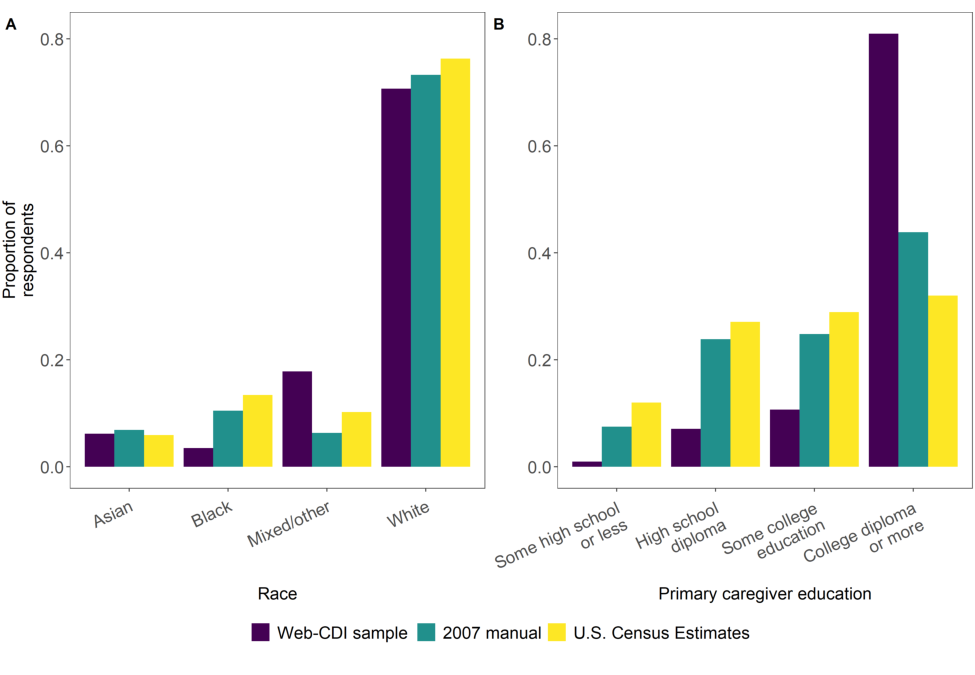
\includegraphics{webcdi_paper_files/figure-latex/demobarfig-1.pdf}
\caption{\label{fig:demobarfig}Proportion of respondents plotted by child race (A) and educational level of primary caregiver (B) from full Web-CDI sample to date (N = 3,524), compared with norming sample demographics from Fenson (2007). Latinx participants can be of any race.}
\end{figure}

\hypertarget{demographic-distribution-and-exclusions}{%
\subsubsection{Demographic distribution and exclusions}\label{demographic-distribution-and-exclusions}}

Figure \ref{fig:demobarfig} shows the distribution of participant ethnicities as compared with previously reported numbers in a large scale norming study of the paper-based CDI form by Fenson et al. (2007). White participants still comprised nearly three quarters of the Web-CDI sample, while a higher proportion of participants report mixed ethnic identification as compared to the 2007 norms. Few participants identified as Hispanic/Latino: 6.5\% of WG participants and 5.1\% of WS participants reported Hispanic of Latino heritage. The low percentage of Hispanic/Latino participants was due in part to our exclusion of children with substantial exposure to languages other than English. Participants' educational attainment level was similarly skewed. Over 80\% of children in the Web-CDI sample came from families with college-educated mothers compared to 43\% from the same group in the 2007 norms (Figure 3). Furthermore, less than 1 percent of participants in our families report a maternal education level less than a high school degree, compared to 7\% from the same group in the 2007 norms. The overrepresentation of white Americans with high levels of education attainment in this sample points to a general challenge encountered in vocabulary development research, which we return to when we detail our efforts to recruit more diverse participants.

\hypertarget{results-to-date}{%
\subsubsection{Results to date}\label{results-to-date}}

\begin{figure}
\centering
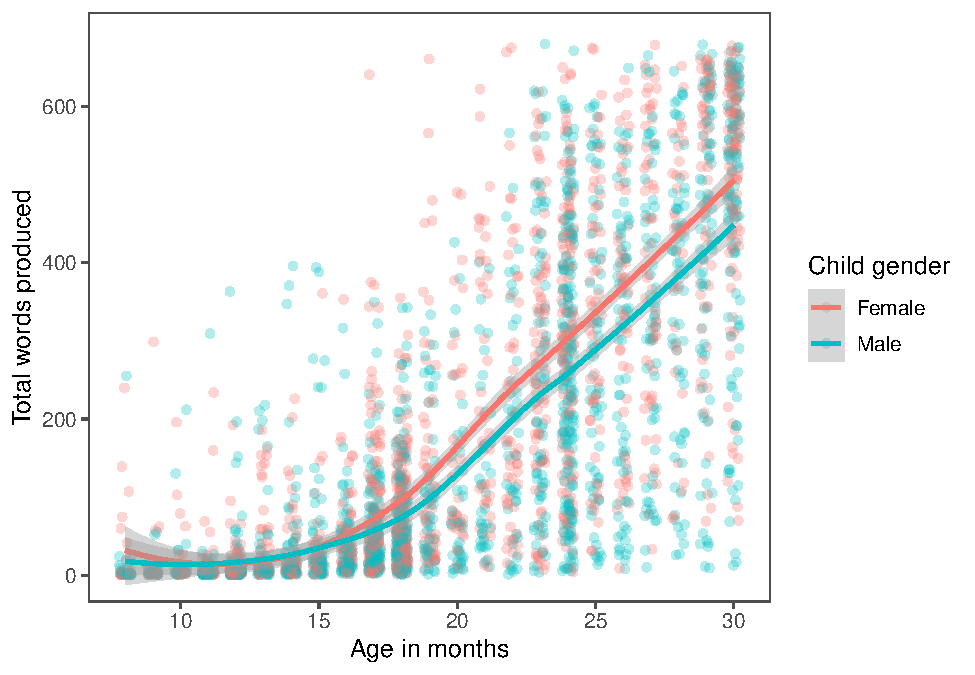
\includegraphics{webcdi_paper_files/figure-latex/genderfig-1.pdf}
\caption{\label{fig:genderfig}Individual children's vocabulary production scores from the entire Web-CDI sample plotted by children's age and gender (both WG and WS, N = 3,513, with 1,674 girls). Line is a locally weighted regression with associated 95\% confidence interval. Children with a different or no reported gender (N = 11) are omitted here.}
\end{figure}

Although the CDI instruments include survey items intended to measure constructs other than vocabulary size, such as gesture, sentence production and grammar, we focus exclusively on the vocabulary measures here. Across both the WG and WS measures, our current Web-CDI sample shows greater reported vocabulary comprehension and production for older children. Moreover, data from both measures replicate a subtle but reliable pattern found in Fenson et al. (1994), (2007) and Feldman et al. (2000) such that female children tend to have slightly larger vocabulary scores than male children across the period of childhood assessed in the CDI forms, though this difference does not appear until the second year of life (Figure \ref{fig:genderfig}).

\begin{figure}
\centering
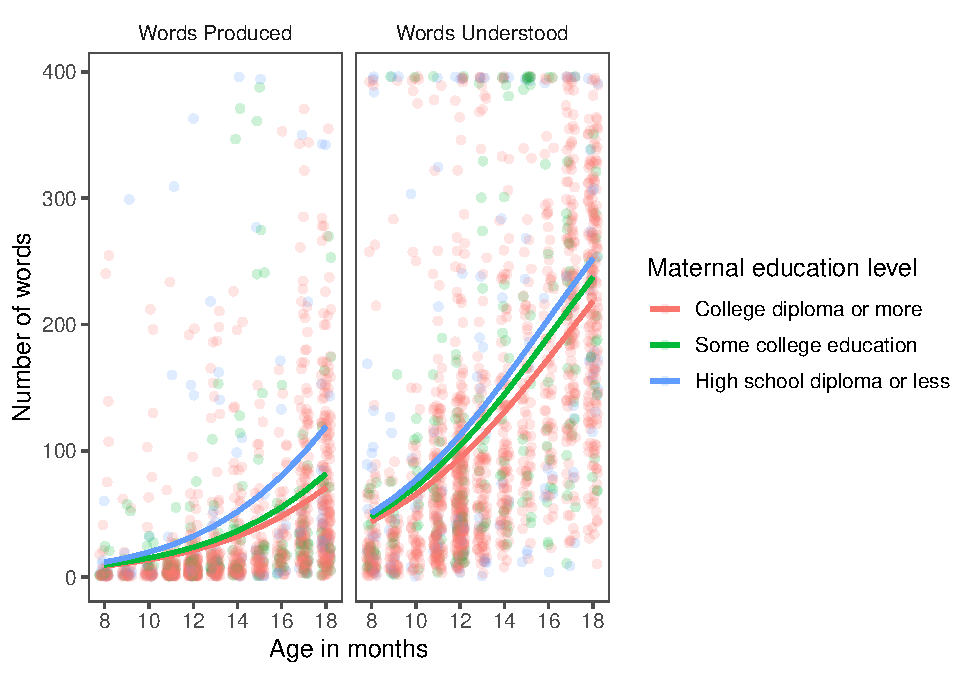
\includegraphics{webcdi_paper_files/figure-latex/wgglm-1.pdf}
\caption{\label{fig:wgglm} Individual children's word production (left panel) and comprehension (right panel) scores plotted by age and primary caregiver's level of education (binned into \enquote{High school diploma or less}, \enquote{Some college education}, and \enquote{College diploma or more}) as reported in the sample of Words and Gestures Web-CDI administrations collected as of November 2020 (N = 1,576). Curves show generalized linear models fits.}
\end{figure}

\begin{figure}
\centering
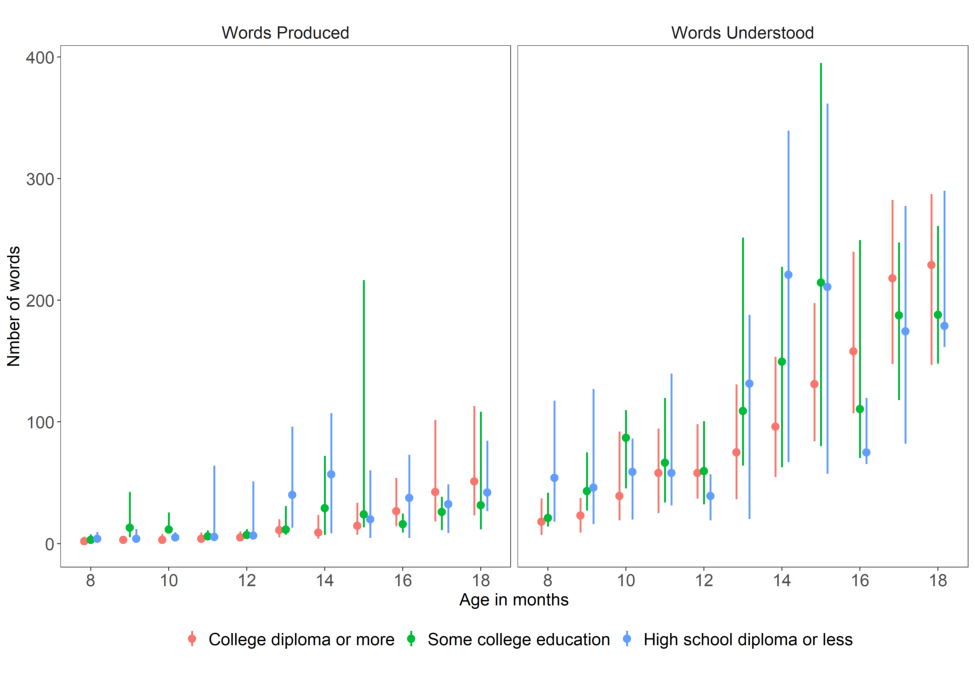
\includegraphics{webcdi_paper_files/figure-latex/wgmedfig-1.pdf}
\caption{\label{fig:wgmedfig}Median vocabulary production (left) and comprehension (right) scores by age on the WG form. Lines indicate span between first and third quartiles for each age.}
\end{figure}

\begin{figure}
\centering
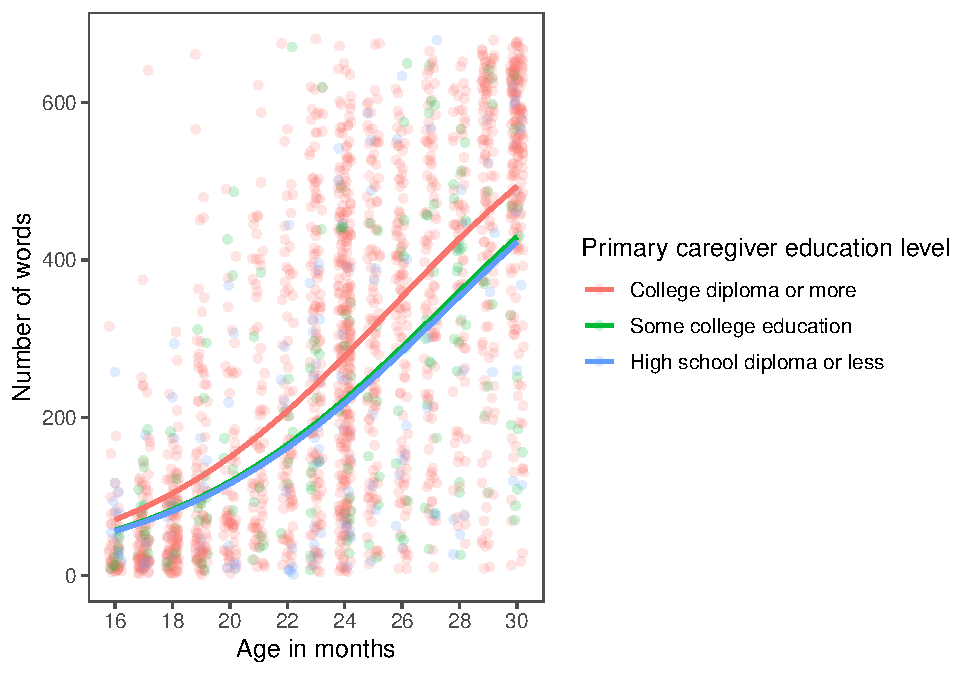
\includegraphics{webcdi_paper_files/figure-latex/wsglm-1.pdf}
\caption{\label{fig:wsglm}Individual children's vocabulary production scores plotted by children's age and maternal education level of primary caregiver education as reported in the sample of Words and Sentences Web-CDI administrations collected as of November 2020 (N = 1,948). Lines are smoothed quantile regressions showing the estimated median vocabulary score within each education group at each age.}
\end{figure}

On the WG form, respondents' reports of children's vocabulary comprehension and production both increased with children's age (Figure \ref{fig:wgglm}). We replicate overall patterns found by Feldman et al. (2000) in that, on both the \enquote{Words Understood} and \enquote{Words Produced} measures, vocabulary scores were slightly negatively correlated with primary caregivers' education level, such that those parents without any college education reported higher vocabulary scores on both scales. A linear regression model with robust standard errors predicting comprehension scores with children's age and primary caregivers' education level (binned into categories of \enquote{High school diploma or less}, \enquote{Some college education} and \enquote{College diploma or more\footnote{``High school diploma'' or less corresponds to 12 or fewer years of education; ``Some college'' corresponds to 13 - 15 years of education; ``College diploma or more'' refers to 16 or more years of education.}}) as predictors shows main effects of both age (\(\beta\) = 19.89, \(p\) \textless{} 0.001) and caregiver primary education (\(\beta_{high school}\) = 29.59, \(p\) = 0.01). Similarly, a linear regression model with robust standard errors predicting production scores by children's age and primary caregivers' education level shows main effects of age (\(\beta\) = 7.82, \(p\) \textless{} 0.001) and caregiver primary education (\(\beta_{high school}\) = 28.86, \(p\) = 0.002).

The pattern of results seen in the WG sample is consistent with prior findings indicating that respondents with lower levels of education attainment report higher vocabulary comprehension and production on the CDI-WG form (Feldman et al., 2000; Fenson et al., 1994). Although caregivers with lower levels of education attainment report higher mean levels of vocabulary production and comprehension, median vocabulary scores show no clear pattern of difference across primary caregiver education levels (Figure \ref{fig:wgmedfig}). This discrepancy between the regression effects and a group-median analysis suggests that the regression effects described previously are driven in part by differential interpretation of the survey items, such that a few lower-SES caregivers are more liberal in reporting their children's productive and comprehensive vocabularies, especially for the youngest children, driving up the mean scores for this demographic group.

Vocabulary production scores on the WS form show the expected pattern of increase with children's age in months; in addition, scores replicate the trend reported in Feldman et al. (2000) such that maternal education is positively associated with children's reported vocabulary size (Figure \ref{fig:wsglm}). Because representation of caregivers without a high school diploma is scarce (N = 18 out of a sample of 1,948), interpretation of the data from this group is constrained. Nevertheless, as shown in Figure \ref{fig:wsglm}, a small but clear positive association between maternal education and vocabulary score exists such that college-educated caregivers report higher vocabulary scores than those of any other education level. The implications from these data converge with previous findings which indicate that parental education levels, often used as a metric of a family's socioeconomic status, are correlated with children's vocabulary size through early childhood.

The data discussed above have stemmed from efforts by many researchers across the United States whose motivations for using the Web-CDI vary. As a result, they reproduce many of the biases of standard US convenience samples. In the next section, we describe in more detail our recent efforts to use the Web-CDI to collect vocabulary development data from traditionally underrepresented participant populations in the United States, attempting to counteract these trends.

\hypertarget{results}{%
\section{Results}\label{results}}

\hypertarget{discussion}{%
\section{Discussion}\label{discussion}}

\newpage

\hypertarget{references}{%
\section{References}\label{references}}

\begingroup
\setlength{\parindent}{-0.5in}
\setlength{\leftskip}{0.5in}

\hypertarget{refs}{}
\leavevmode\hypertarget{ref-Alcock2020}{}%
Alcock, K., Meints, K., Rowland, C., \& others. (2020). \emph{The uk communicative development inventories: Words and gestures}. J\&R Press.

\leavevmode\hypertarget{ref-Bates2001}{}%
Bates, E., \& Goodman, J. C. (2001). On the inseparability of grammar and the lexicon: Evidence from acquisition.

\leavevmode\hypertarget{ref-bates1994}{}%
Bates, E., Marchman, V., Thal, D., Fenson, L., Dale, P., Reznick, J. S., \ldots{} Hartung, J. (1994). Developmental and stylistic variation in the composition of early vocabulary. \emph{J Child Lang}, \emph{21}(01), 85--123.

\leavevmode\hypertarget{ref-bornstein2012}{}%
Bornstein, M. H., \& Putnick, D. L. (2012). Stability of language in childhood: A multiage, multidomain, multimeasure, and multisource study. \emph{Developmental Psychology}, \emph{48}(2), 477.

\leavevmode\hypertarget{ref-Caselli2020}{}%
Caselli, N. K., Lieberman, A. M., \& Pyers, J. E. (2020). The asl-cdi 2.0: An updated, normed adaptation of the macarthur bates communicative development inventory for american sign language. \emph{Behavior Research Methods}, 1--14.

\leavevmode\hypertarget{ref-dale2015}{}%
Dale, P. S. (2015). Adaptations, Not Translations! Retrieved from \url{http://mb-cdi.stanford.edu/Translations2015.pdf}

\leavevmode\hypertarget{ref-feldman2000}{}%
Feldman, H. M., Dollaghan, C. A., Campbell, T. F., Kurs-Lasky, M., Janosky, J. E., \& Paradise, J. L. (2000). Measurement properties of the macarthur communicative development inventories at ages one and two years. \emph{Child Development}, \emph{71}(2), 310--322.

\leavevmode\hypertarget{ref-fenson2007}{}%
Fenson, L., Bates, E., Dale, P. S., Marchman, V. A., Reznick, J. S., \& Thal, D. J. (2007). \emph{MacArthur-Bates Communicative Development Inventories}. Brookes Publishing Company.

\leavevmode\hypertarget{ref-fenson1994}{}%
Fenson, L., Dale, P. S., Reznick, J. S., Bates, E., Thal, D. J., Pethick, S. J., \ldots{} Stiles, J. (1994). Variability in early communicative development. \emph{Monogr Soc Res Child Dev}, \emph{59}(5).

\leavevmode\hypertarget{ref-fenson2000b}{}%
Fenson, L., Pethick, S., Renda, C., Cox, J. L., Dale, P. S., \& Reznick, J. S. (2000). Short-form versions of the macarthur communicative development inventories. \emph{Applied Psycholinguistics}, \emph{21}(1), 95--116.

\leavevmode\hypertarget{ref-Frank2021}{}%
Frank, M. C., Braginsky, M., Yurovsky, D., \& Marchman, V. A. (2021). \emph{Variability and consistency in early language learning: The wordbank project}. MIT Press.

\leavevmode\hypertarget{ref-kristoffersen2013}{}%
Kristoffersen, K. E., Simonsen, H. G., Bleses, D., Wehberg, S., Jørgensen, R. N., Eiesland, E. A., \& Henriksen, L. Y. (2013). The use of the internet in collecting cdi data--an example from norway. \emph{Journal of Child Language}, \emph{40}(03), 567--585.

\endgroup


\end{document}
